% Options for packages loaded elsewhere
\PassOptionsToPackage{unicode}{hyperref}
\PassOptionsToPackage{hyphens}{url}
%
\documentclass[
]{article}
\title{Uncertainty in times of COVID-19: Choosing whether to ask 1 or 2
questions}
\author{Fabian Lange, Lars Vilhuber}
\date{2022-06-03}

\usepackage{amsmath,amssymb}
\usepackage{lmodern}
\usepackage{iftex}
\ifPDFTeX
  \usepackage[T1]{fontenc}
  \usepackage[utf8]{inputenc}
  \usepackage{textcomp} % provide euro and other symbols
\else % if luatex or xetex
  \usepackage{unicode-math}
  \defaultfontfeatures{Scale=MatchLowercase}
  \defaultfontfeatures[\rmfamily]{Ligatures=TeX,Scale=1}
\fi
% Use upquote if available, for straight quotes in verbatim environments
\IfFileExists{upquote.sty}{\usepackage{upquote}}{}
\IfFileExists{microtype.sty}{% use microtype if available
  \usepackage[]{microtype}
  \UseMicrotypeSet[protrusion]{basicmath} % disable protrusion for tt fonts
}{}
\makeatletter
\@ifundefined{KOMAClassName}{% if non-KOMA class
  \IfFileExists{parskip.sty}{%
    \usepackage{parskip}
  }{% else
    \setlength{\parindent}{0pt}
    \setlength{\parskip}{6pt plus 2pt minus 1pt}}
}{% if KOMA class
  \KOMAoptions{parskip=half}}
\makeatother
\usepackage{xcolor}
\IfFileExists{xurl.sty}{\usepackage{xurl}}{} % add URL line breaks if available
\IfFileExists{bookmark.sty}{\usepackage{bookmark}}{\usepackage{hyperref}}
\hypersetup{
  pdftitle={Uncertainty in times of COVID-19: Choosing whether to ask 1 or 2 questions},
  pdfauthor={Fabian Lange, Lars Vilhuber},
  hidelinks,
  pdfcreator={LaTeX via pandoc}}
\urlstyle{same} % disable monospaced font for URLs
\usepackage[margin=1in]{geometry}
\usepackage{longtable,booktabs,array}
\usepackage{calc} % for calculating minipage widths
% Correct order of tables after \paragraph or \subparagraph
\usepackage{etoolbox}
\makeatletter
\patchcmd\longtable{\par}{\if@noskipsec\mbox{}\fi\par}{}{}
\makeatother
% Allow footnotes in longtable head/foot
\IfFileExists{footnotehyper.sty}{\usepackage{footnotehyper}}{\usepackage{footnote}}
\makesavenoteenv{longtable}
\usepackage{graphicx}
\makeatletter
\def\maxwidth{\ifdim\Gin@nat@width>\linewidth\linewidth\else\Gin@nat@width\fi}
\def\maxheight{\ifdim\Gin@nat@height>\textheight\textheight\else\Gin@nat@height\fi}
\makeatother
% Scale images if necessary, so that they will not overflow the page
% margins by default, and it is still possible to overwrite the defaults
% using explicit options in \includegraphics[width, height, ...]{}
\setkeys{Gin}{width=\maxwidth,height=\maxheight,keepaspectratio}
% Set default figure placement to htbp
\makeatletter
\def\fps@figure{htbp}
\makeatother
\setlength{\emergencystretch}{3em} % prevent overfull lines
\providecommand{\tightlist}{%
  \setlength{\itemsep}{0pt}\setlength{\parskip}{0pt}}
\setcounter{secnumdepth}{-\maxdimen} % remove section numbering
\ifLuaTeX
  \usepackage{selnolig}  % disable illegal ligatures
\fi

\begin{document}
\maketitle

{
\setcounter{tocdepth}{2}
\tableofcontents
}
\hypertarget{purpose}{%
\subsection{Purpose}\label{purpose}}

We fielded three questions regarding uncertainty in the April 2020
COVID-19 situation in Canada. Goal is to select either a two-question
survey, using different questions for employment and consumer behavior,
or a composite question that encompasses both. The question is whether
answers between the two-question version differ between questions. The
composite question was asked as a control.

\hypertarget{sources}{%
\subsection{Sources}\label{sources}}

We \href{https://osf.io/729nr}{pre-registered} the decision based on
\textbf{preliminary data} collected after the first day of fielding the
question (on 20200421). The decision about choice of the question, as
well as preliminary descriptive results, are based on \textbf{test data}
collected over the entire test time period, with a target n of 250 per
question. We collected data from 2020-04-12 to 2020-04-17 across Canada,
achieving a total \emph{n}=753.

The data was manually downloaded from the Google Consumer Survey site on
20200412, and saved, using the naming convention
\texttt{tag-YYYYMMDD-HHMM.xlsx}. Data used for both the original design
and the full test time period are available in this archive.

\hypertarget{preliminary-data-files}{%
\subsubsection{Preliminary data files}\label{preliminary-data-files}}

\includegraphics{evaluation_files/figure-latex/list_test_files-1.pdf}

\hypertarget{test-data-files}{%
\subsubsection{Test data files}\label{test-data-files}}

\includegraphics{evaluation_files/figure-latex/list_prelim_files-1.pdf}

\hypertarget{fielded-questions}{%
\subsection{Fielded questions}\label{fielded-questions}}

We fielded three questions in the test sample:

\begin{itemize}
\tightlist
\item
  How much longer do you expect social distancing rules (restrictions on
  gatherings, stay-at-home rules) to stay in place in your province?
\item
  How much longer do you expect the closure of non-essential businesses
  to stay in place in your province?
\item
  How much longer do you expect social distancing rules (restrictions on
  gatherings, closure of non-essential businesses, stay-at-home rules)
  to stay in place in your province?
\end{itemize}

For each question, we collected responses on a Likert scale with text:
``less than 1 month'', ``1-2 months'', ``2-3 months'', ``3-6 months'',
``more than 6 months'', and a response equivalent to ``does not apply''
(``My province has not implemented such rules.'').

\hypertarget{first-results}{%
\subsection{First results}\label{first-results}}

\hypertarget{total-observation-by-tag-question}{%
\subsubsection{Total observation by tag /
question}\label{total-observation-by-tag-question}}

\begin{verbatim}
## `summarise()` has grouped output by 'tag'. You can override using the `.groups`
## argument.
\end{verbatim}

\begin{longtable}[]{@{}llr@{}}
\toprule
tag & date & count \\
\midrule
\endhead
business & 20200421 & 251 \\
composite & 20200421 & 251 \\
people & 20200421 & 251 \\
\bottomrule
\end{longtable}

\hypertarget{responses-to-question-1}{%
\subsubsection{Responses to Question 1}\label{responses-to-question-1}}

\begin{longtable}[]{@{}lrr@{}}
\toprule
Q1 & count & percent \\
\midrule
\endhead
less than 1 month & 25 & 9.96 \\
1-2 months & 77 & 30.68 \\
2-3 months & 55 & 21.91 \\
3-6 months & 39 & 15.54 \\
more than 6 months & 37 & 14.74 \\
My province has not implemented such rules. & 18 & 7.17 \\
\bottomrule
\end{longtable}

\hypertarget{responses-to-question-2}{%
\subsubsection{Responses to Question 2}\label{responses-to-question-2}}

\begin{longtable}[]{@{}lrr@{}}
\toprule
Q1 & count & percent \\
\midrule
\endhead
less than 1 month & 28 & 11.16 \\
1-2 months & 74 & 29.48 \\
2-3 months & 54 & 21.51 \\
3-6 months & 44 & 17.53 \\
more than 6 months & 24 & 9.56 \\
My province has not implemented such rules. & 27 & 10.76 \\
\bottomrule
\end{longtable}

\hypertarget{responses-to-question-3}{%
\subsubsection{Responses to Question 3}\label{responses-to-question-3}}

\begin{longtable}[]{@{}lrr@{}}
\toprule
Q1 & count & percent \\
\midrule
\endhead
less than 1 month & 24 & 9.56 \\
1-2 months & 69 & 27.49 \\
2-3 months & 55 & 21.91 \\
3-6 months & 38 & 15.14 \\
more than 6 months & 37 & 14.74 \\
My province has not implemented such rules. & 28 & 11.16 \\
\bottomrule
\end{longtable}

\hypertarget{do-the-different-questions-yield-different-responses}{%
\subsection{Do the different questions yield different
responses?}\label{do-the-different-questions-yield-different-responses}}

\hypertarget{visually}{%
\subsubsection{Visually}\label{visually}}

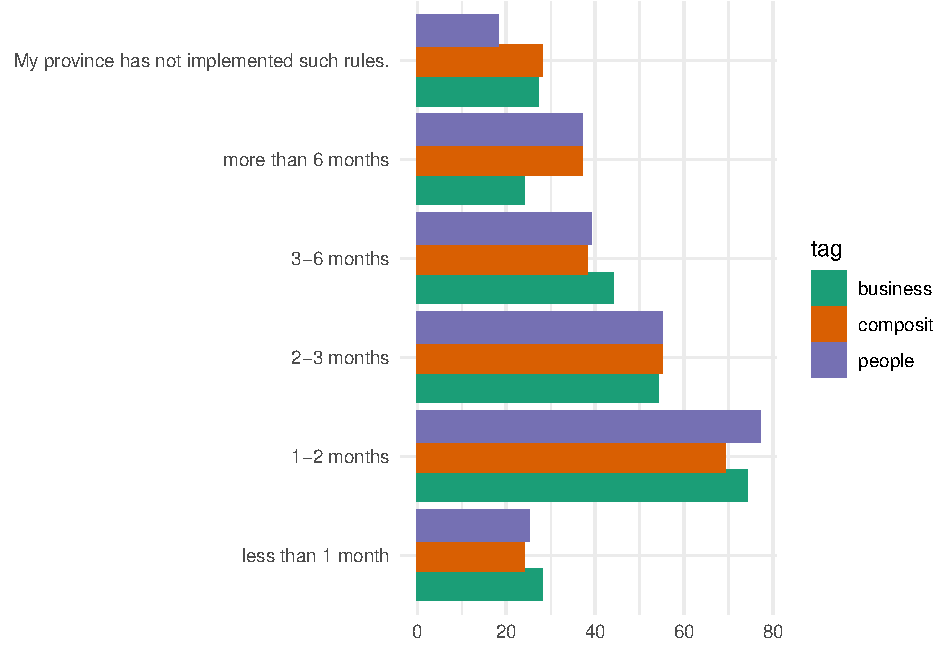
\includegraphics{evaluation_files/figure-latex/graph-1.pdf}

\hypertarget{kolmogorov-smirnov-test}{%
\subsubsection{Kolmogorov-Smirnov Test}\label{kolmogorov-smirnov-test}}

\begin{verbatim}
## `summarise()` has grouped output by 'tag'. You can override using the `.groups`
## argument.
\end{verbatim}

\begin{verbatim}
## 
##  Two-sample Kolmogorov-Smirnov test
## 
## data:  hist.business and hist.people
## D = 0.16667, p-value = 1
## alternative hypothesis: two-sided
\end{verbatim}

In the Kolmogorov-Smirnov test, the entire (cumulative) distribution is
tested for equality. The hypothesis of equality of distributions is
rejected when the test statistic \(D\) is larger than
\(c(\alpha) \sqrt{\frac{n+m}{n*m}}\) where \(n\) and \(m\) are the
sample sizes.

For the full test data, \(n=\) 251 and \(m=\) 251, the square root
evaluates to 0.0892644. The test statistic \(D=\) 0.1666667, with a
p-value of 1. Based on the KS test, we thus reject the hypothesis of
equality of distributions.

\hypertarget{single-dimensional-test}{%
\subsubsection{Single-dimensional test}\label{single-dimensional-test}}

Alternatively, we can compute a \(z\)-test for the proportion responding
to Q1 with ``1-2 months'', with the remaining fractions collapsed to an
``other'' category. For the test sample, these numbers are 29.4820717
percent for the \texttt{business} version, and 30.6772908 percent for
the \texttt{people} version. The \(\chi^2\) statistic has a value of
0.0378861 and a p-value of 0.8456721. Based on the \(z\)-test, we cannot
reject the hypothesis of equality of responses to Q1. For the
(non-pre-registered) comparison of the fraction responding with ``more
than 6 months'', the \(\chi^2\) statistic has a value of 2.6871863 and a
p-value of 0.1011583.

The test has power of 0.05 for the sample size n=251 and effect size
9.56 at \(\alpha =\) 0.05.

\hypertarget{fishers-exact-test}{%
\subsubsection{Fisher's exact test}\label{fishers-exact-test}}

\begin{verbatim}
## 
##  Fisher's Exact Test for Count Data with simulated p-value (based on
##  10000 replicates)
## 
## data:  hist.business and hist.people
## p-value = 1
## alternative hypothesis: two.sided
\end{verbatim}

We can also use Fisher's exact test to assess whether the two
distributions are different. The null hypothesis is that the rows
\emph{and} columns of the two histograms are independent (i.e., the two
distributions are different). Fisher's test when applied to the test
sample gives a p-value of 1, so the null that the two distributions are
different should be rejected.

\hypertarget{chi2-test}{%
\subsubsection{\texorpdfstring{\(\chi^2\)
test}{\textbackslash chi\^{}2 test}}\label{chi2-test}}

\begin{verbatim}
## 
##  Pearson's Chi-squared test with simulated p-value (based on 10000
##  replicates)
## 
## data:  hist.business and hist.people
## X-squared = 30, df = NA, p-value = 1
\end{verbatim}

Finally, a \(\chi^2\) test of independence of distributions yields a
test statistic of 30 and a p-value of 1, not rejecting the null that the
two histograms are different.

\hypertarget{decision-criterion}{%
\subsection{Decision Criterion}\label{decision-criterion}}

We will use one composite question if the two variants
(\texttt{business} and \texttt{people}) are not statistically different
in our test sample, according to the majority of tests.

\hypertarget{results}{%
\subsection{Results}\label{results}}

Based on the observed data from the test data collected between
2020-04-12 and 2020-04-17 across Canada, we chose the two-question
version.

\hypertarget{license}{%
\subsection{License}\label{license}}

This text and the underlying data are licensed under a
\href{https://creativecommons.org/licenses/by-nc/4.0/}{Creative Commons
Attribution-NonCommercial 4.0 International} license.

\end{document}
